After the process of feature selection was completed parameter training by means of Stochastic Gradient Descent could take place. Values of the trained weights are presented in table \ref{table:weights_nonlinear_noise_free}.
\npdecimalsign{.}
\nprounddigits{5}
\begin{table}[ht]
\caption{Trained weights for segmentation of noise free images.}
\centering
\begin{tabular}{|c|c|c|}
\hline
\rowcolor[HTML]{C0C0C0} 
$w_1$(unary potential) & $w_{2,1}$ (pairwise potential) & $w_{2,2}$ (bias) \\ \hline
?? & ?? & ?? \\ \hline
\end{tabular}
\label{table:weights_nonlinear_noise_free}
\end{table}

Having a parametrised model it was possible to perform inference on the set of unknown test samples. Figure \ref{fig:nonlinear_results_noise_free} presents the results of the semantic segmentation process on sample test images. In the first column an original image that is to be segmented is showed. The next two columns depict segmentation results, with only local potential, and with both potentials involved. The last column presents the expected results.  

\begin{figure}[!htb]
 \centering
    \begin{tabular}{cccc}
        \textit{sample image} & \textit{local potential} & \textit{experimental result} & \textit{expected results} \\

       \fcolorbox{black}{white}{\includegraphics[width = 0.20\textwidth]{nonlinear_noise_free/experiments/init/17.png}} &
       \fcolorbox{black}{white}{\includegraphics[width = 0.20\textwidth]{nonlinear_noise_free/experiments/only_fi1/17.png}} &
        \fcolorbox{black}{white}{
\includegraphics[width = 0.20\textwidth]{placeholder.png}} &
        \fcolorbox{black}{white}{\includegraphics[width = 0.20\textwidth]{nonlinear_noise_free/experiments/ground_truth/17.png}} \\
        \fcolorbox{black}{white}{\includegraphics[width = 0.20\textwidth]{nonlinear_noise_free/experiments/init/19.png}} &
       \fcolorbox{black}{white}{\includegraphics[width = 0.20\textwidth]{nonlinear_noise_free/experiments/only_fi1/19.png}} &
        \fcolorbox{black}{white}{
\includegraphics[width = 0.20\textwidth]{placeholder.png}} &
        \fcolorbox{black}{white}{\includegraphics[width = 0.20\textwidth]{nonlinear_noise_free/experiments/ground_truth/19.png}} \\
        \fcolorbox{black}{white}{
\includegraphics[width = 0.20\textwidth]{nonlinear_noise_free/experiments/init/20.png}} &
        \fcolorbox{black}{white}{
\includegraphics[width = 0.20\textwidth]{nonlinear_noise_free/experiments/only_fi1/20.png}} &
        \fcolorbox{black}{white}{
\includegraphics[width = 0.20\textwidth]{placeholder.png}} &
        \fcolorbox{black}{white}{
\includegraphics[width = 0.20\textwidth]{nonlinear_noise_free/experiments/ground_truth/20.png}} \\
        \fcolorbox{black}{white}{\includegraphics[width = 0.20\textwidth]{nonlinear_noise_free/experiments/init/23.png}} &
        \fcolorbox{black}{white}{\includegraphics[width = 0.20\textwidth]{nonlinear_noise_free/experiments/only_fi1/23.png}} &
        \fcolorbox{black}{white}{
\includegraphics[width = 0.20\textwidth]{placeholder.png}} &
        \fcolorbox{black}{white}{\includegraphics[width = 0.20\textwidth]{nonlinear_noise_free/experiments/ground_truth/23.png}} \\
        \fcolorbox{black}{white}{\includegraphics[width = 0.20\textwidth]{nonlinear_noise_free/experiments/init/7.png}} &
        \fcolorbox{black}{white}{\includegraphics[width = 0.20\textwidth]{nonlinear_noise_free/experiments/only_fi1/7.png}} &
        \fcolorbox{black}{white}{
\includegraphics[width = 0.20\textwidth]{placeholder.png}} &
        \fcolorbox{black}{white}{\includegraphics[width = 0.20\textwidth]{nonlinear_noise_free/experiments/ground_truth/7.png}} \\
    \end{tabular}
    \caption{Experimental results of semantic image segmentation on sample multicoloured images in RGB colour space.}
    \label{fig:nonlinear_results_noise_free}
\end{figure}

[...]
 TODO: \textit{description of the results} 
[...]

The accuracy of semantic segmentation on images with objects of different shapes is in the table \ref{table:iou_nonlinear_noise_free}. [...]
\begin{table}[ht]
\centering
\caption{Accuracy of segmentation based on shape detection for noise free data.}
\label{table:iou_nonlinear_noise_free}
    \begin{tabular}{|
    >{\columncolor[HTML]{9B9B9B}}c|c|c|c|c|
    >{\columncolor[HTML]{343434}}c|}
    \hline
    \textit{class} & \cellcolor[HTML]{9B9B9B}label 0 & \cellcolor[HTML]{9B9B9B}label 1 & \cellcolor[HTML]{9B9B9B}label 2 &  \cellcolor[HTML]{9B9B9B}label 3 & {\color[HTML]{FFFFFF} mIoU {[}\%{]}} \\ \hline
    local potential IoU {[}\%{]} & 97.89 & 99.95 & 99.91 & 95.51 &{\color[HTML]{FFFFFF} 98.32} \\ \hline
    final IoU {[}\%{]} & ?? & ?? & ?? & ?? &{\color[HTML]{FFFFFF} ??} \\ \hline
    \end{tabular}
\end{table}